% ADMA 2026 submission — Springer LNCS/LNAI format.
% Requires llncs.cls and splncs04.bst from the Springer LNCS template
% (see paper/README.md). Compile: pdflatex -> bibtex -> pdflatex x2.
\documentclass[runningheads]{llncs}

\usepackage[T1]{fontenc}
\usepackage{graphicx}
\usepackage{amsmath,amssymb}
\usepackage{booktabs}
\usepackage{multirow}
\usepackage{url}
\usepackage{tikz}
\usepackage{xcolor}
\usetikzlibrary{positioning,arrows.meta,fit,backgrounds}

\newcommand{\model}{DD-Mamba}
\newcommand{\best}[1]{\textbf{#1}}
\newcommand{\second}[1]{\underline{#1}}

% ADMA review is DOUBLE-BLIND: keep \anonymoustrue for the submission.
% Flip to \anonymousfalse (and fill in the real author block below) only
% for the camera-ready version.
\newif\ifanonymous
\anonymoustrue

\begin{document}

\title{\model{}: A Dual-Domain State-Space Forecasting Framework with
Linear Anchors and Zero-Initialized Corrections}
\titlerunning{Dual-Domain State-Space Forecasting}

\ifanonymous
\author{Anonymous Submission}
\authorrunning{Anonymous Submission}
\institute{ADMA 2026 double-blind review}
\else
% TODO: replace with the real author list for the camera-ready.
\author{First Author\inst{1}\orcidID{0000-0000-0000-0000} \and
Second Author\inst{1}}
\authorrunning{F. Author et al.}
\institute{Affiliation, City, Country\\
\email{first.author@example.edu}}
\fi

\maketitle

\begin{abstract}
Long-term multivariate time series forecasting must reconcile two
complementary views: local, trend-driven dynamics in the time
domain, and global periodic structure most compact in the frequency
domain. Existing state-space (Mamba) forecasters model one view but
not both, and deep forecasters often discard simple linear maps that
remain near state-of-the-art. We
present \model{}, a dual-domain forecasting \emph{framework} whose time
branch (decomposition with a selective state-space encoder) and
frequency branch (learned spectral filtering) each produce a forecast,
fused by a convex gate that preserves both prediction
paths. Two principles organize the
framework: (i)~\emph{linear anchoring} --- the time branch carries a
DLinear-style linear pathway, the frequency branch an optional FITS-style
spectral map, and all nonlinear heads are zero-initialized, so at
initialization the model reduces to a linear map of the
instance-normalized window; and (ii)~\emph{capacity placement} --- a bidirectional
Mamba over the \emph{variate} dimension carries the model on high-channel
data and is disabled on few-channel data where it overfits. On nine benchmarks under the look-back-96 protocol (three
seeds), \model{} reports the lowest mean MSE on seven, improving over
reported S-Mamba results on five (up to 17\% on Solar), tying three
within noise, and trailing one, with fewer parameters on small
datasets. Paired three-seed ablations on three datasets validate capacity
placement in both directions (the variate mixer helps weather yet hurts
ETTh1; normalization helps weather yet hurt solar), show a significant
frequency-branch contribution on Solar with redundancy elsewhere, and
find zero initialization accuracy-neutral; dual-domain modeling is a
per-dataset structural option, not a universal gain.
\keywords{Time series forecasting \and State-space models \and Mamba \and
Frequency domain \and Multivariate analysis}
\end{abstract}

\section{Introduction}

Long-term forecasting of multivariate time series underpins applications
from power-grid load planning to traffic management and weather-dependent
operations. The field has cycled through architectural paradigms at a
remarkable pace: Transformer variants with efficient attention
\cite{informer,autoformer,fedformer}, patch-based attention
\cite{patchtst}, inverted variate-token attention \cite{itransformer},
and, most recently, selective state-space models (SSMs) built on Mamba
\cite{mamba,smamba}, which offer linear-time sequence modeling with
input-dependent dynamics.

\emph{Three empirical gaps} complicate this progress. \textbf{Gap~1: deep
models discard strong linear maps.} A per-component linear projection from
the look-back window to the horizon (DLinear \cite{dlinear}) and a tiny
complex-linear interpolation of the low-passed spectrum (FITS \cite{fits})
match or beat far larger models on several benchmarks, especially the ETT
family; deep architectures that ignore this spend their early training
re-discovering a linear map, and on small datasets often never do.
\textbf{Gap~2: the useful inductive bias differs by domain.} Local trends
and regime changes are naturally expressed in the time domain, while
multi-scale seasonality is compact in the frequency domain, yet models
committed to a single view --- attention or SSMs over time steps only, or
spectral mixing only \cite{frets} --- systematically underuse the other.
\textbf{Gap~3: the right amount of capacity is dataset-dependent.}
Cross-variate mixing is the decisive component on high-dimensional
benchmarks \cite{itransformer,smamba} yet pure overfitting capacity on
low-channel data, so any \emph{fixed} architecture is mis-sized for one
regime or the other.

We answer these three gaps with \model{} (Fig.~\ref{fig:arch}), mapping
each to one structural remedy (Fig.~\ref{fig:gaps}): \emph{(i)}~an explicit
linear anchor with zero-initialized nonlinear corrections in each branch;
\emph{(ii)}~parallel time and frequency branches, fused by a convex gate
that preserves both prediction paths; and \emph{(iii)}~a bidirectional
variate mixer switched on or off per dataset. Each remedy is detailed
below.

\begin{figure}[t]
\centering
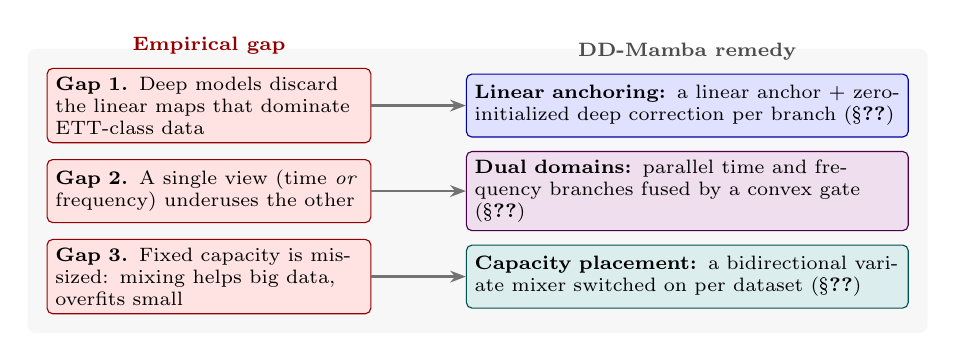
\begin{tikzpicture}[
  font=\scriptsize,
  gap/.style={draw=red!58!black, fill=red!11, rounded corners=2pt,
              align=left, text width=39mm, inner sep=3pt, minimum height=8mm},
  remb/.style={draw=blue!62!black, fill=blue!12, rounded corners=2pt,
               align=left, text width=54mm, inner sep=3pt, minimum height=8mm},
  remv/.style={draw=violet!60!black, fill=violet!13, rounded corners=2pt,
               align=left, text width=54mm, inner sep=3pt, minimum height=8mm},
  remt/.style={draw=teal!62!black, fill=teal!14, rounded corners=2pt,
               align=left, text width=54mm, inner sep=3pt, minimum height=8mm},
  to/.style={-{Stealth[length=2mm]}, thick, black!55}]

\node[gap] (g1) {\textbf{Gap 1.} Deep models discard the linear maps that
  dominate ETT-class data};
\node[gap, below=2mm of g1] (g2) {\textbf{Gap 2.} A single view (time
  \emph{or} frequency) underuses the other};
\node[gap, below=2mm of g2] (g3) {\textbf{Gap 3.} Fixed capacity is
  mis-sized: mixing helps big data, overfits small};

\node[remb, right=12mm of g1] (r1) {\textbf{Linear anchoring:} a linear
  anchor $+$ zero-initialized deep correction per branch (\S\ref{sec:anchors})};
\node[remv, right=12mm of g2] (r2) {\textbf{Dual domains:} parallel time
  and frequency branches fused by a convex gate (\S\ref{sec:fusion})};
\node[remt, right=12mm of g3] (r3) {\textbf{Capacity placement:} a
  bidirectional variate mixer switched on per dataset (\S\ref{sec:mixer})};

\draw[to] (g1) -- (r1);
\draw[to] (g2) -- (r2);
\draw[to] (g3) -- (r3);

\node[font=\scriptsize\bfseries, above=0.5mm of g1, red!58!black] {Empirical gap};
\node[font=\scriptsize\bfseries, above=0.5mm of r1, black!70] {\model{} remedy};

\begin{scope}[on background layer]
  \node[fill=black!3, rounded corners=3pt, inner sep=2.4mm,
        fit=(g1)(g3)(r1)(r3)] {};
\end{scope}
\end{tikzpicture}
\caption{The three empirical gaps that motivate \model{} and the remedy
each maps to, colour-matched to Fig.~\ref{fig:arch}:
\textcolor{blue!62!black}{time/linear} (blue),
\textcolor{violet!60!black}{dual-domain fusion} (violet), and
\textcolor{teal!62!black}{capacity placement} (teal).}
\label{fig:gaps}
\end{figure}

\textbf{Dual branches with structurally preserved paths.} A time and a
frequency branch each output a complete forecast; the model's prediction
is their learned \emph{convex combination}, the gate conditioned on both
branches' features. Constrained elementwise between the two forecasts,
both domains keep an explicit prediction path, and the gate value reports
each branch's convex weight --- a proxy for, not a causal measure of, its
contribution --- while the gate may saturate near 0 or 1 and lean almost
entirely on one branch. Our paired ablations find the frequency branch
significant on one of three ablated datasets (Solar) and within noise on
the others (Sect.~\ref{sec:ablation}); we thus claim per-dataset
flexibility, not a universal dual-domain gain.

\textbf{Linear anchors with zero-initialized corrections.} Each branch
carries an explicit \emph{linear} pathway of its domain --- DLinear-style
seasonal/trend projections \cite{dlinear} in the time branch, an optional
FITS-style complex-linear spectral map \cite{fits} in the frequency branch
--- trained jointly, not pretrained. All nonlinear heads (and the spectral
map) are zero-initialized and the gate opens at a constant $g_0$, so at
initialization the model reduces to $g_0$ times a randomly initialized
DLinear-style map of the \emph{instance-normalized} window
(Sect.~\ref{sec:anchors}), the same normalization wrapper as RLinear-class
models \cite{rlinear,revin}. A controlled comparison against random
initialization finds this accuracy-neutral (Sect.~\ref{sec:ablation}), so
we position it as an interpretability default, not an accuracy mechanism.

\textbf{Mamba where it pays.} A causal Mamba encoder models the time axis;
a \emph{bidirectional} Mamba (frequency bins and channels have no arrow of
time) optionally does spectral encoding and cross-variate mixing in the
spirit of S-Mamba \cite{smamba}. Capacity is \emph{placed} per dataset,
and the paired ablations support this in both directions: removing the
variate mixer hurts weather while \emph{adding} it hurts ETTh1, each with
a CI excluding zero (Sect.~\ref{sec:ablation}).

Our contributions are:
\begin{enumerate}
\item A dual-domain forecasting architecture whose output is a gated
convex combination of per-branch forecasts, structurally preserving a
prediction path from each domain and exposing each branch's per-sample
convex weight (Sect.~\ref{sec:method}).
\item A linear-anchoring scheme --- domain-appropriate linear pathways
with zero-initialized nonlinear corrections --- under which the model at
initialization reduces to a linear map of the instance-normalized window;
a controlled comparison against random initialization finds it
accuracy-neutral, so its value is the interpretable linear start
(Sect.~\ref{sec:anchors}, Sect.~\ref{sec:ablation}).
\item A capacity-placement recipe for selective SSMs: causal Mamba over
time where temporal microstructure matters, bidirectional Mamba over
variates where cross-channel structure dominates, and neither where data
is scarce (Sect.~\ref{sec:mixer}).
\item The lowest reported average MSE on seven of nine standard
benchmarks under the unified look-back-96 protocol (three-seed
mean~$\pm$~std for every entry), relative to results published under the
same protocol, plus a released ablation harness and paired multi-seed ablations
on three datasets --- including negative and dataset-dependent findings
(instance normalization helps weather and traffic yet hurts solar) that
we believe are as actionable as the positive ones
(Sect.~\ref{sec:experiments}).
\end{enumerate}

\section{Related Work}

\paragraph{Transformer forecasters.} Informer \cite{informer}, Autoformer
\cite{autoformer} and FEDformer \cite{fedformer} adapt attention to long
sequences via sparsity, decomposition, and frequency-domain mixing
respectively. PatchTST \cite{patchtst} treats sub-series patches as tokens
with channel independence; iTransformer \cite{itransformer} inverts the
axes and attends over \emph{variates}, establishing that cross-channel
modeling, not temporal attention, drives accuracy on high-dimensional
benchmarks. \model{} adopts the variate-mixing insight but implements it
with linear-time bidirectional SSMs and, unlike these works, couples it to
an explicit frequency branch and linear anchors.

\paragraph{Linear and frequency-domain models.} DLinear/NLinear \cite{dlinear}
showed that decomposition plus a linear map rivals Transformers,
particularly on ETT; RLinear \cite{rlinear} added reversible instance
normalization \cite{revin}. FreTS \cite{frets} learns MLPs in the
frequency domain, and FITS \cite{fits} forecasts with a single complex
linear interpolation of the low-passed spectrum at negligible parameter
cost. \model{} does not compete with these models --- it \emph{contains}
them: each branch carries a linear pathway of its domain's model family,
and the deep machinery is trained as a correction on top.

\paragraph{State-space models.} Mamba \cite{mamba} introduced selective SSMs
with input-dependent dynamics and linear-time scans. In forecasting,
S-Mamba \cite{smamba} applies bidirectional Mamba over variate tokens with
a linear temporal embedding, and further works explore frequency-domain
SSMs \cite{fmamba}. \model{} unifies these threads: causal Mamba over
time, bidirectional Mamba over frequency bins and over variates, with the
placement of each governed by dataset characteristics rather than applied
uniformly.

\paragraph{Decomposition and heteroscedasticity.} Splitting a series into
interpretable components is a century-old idea: classical additive and
multiplicative models, STL, wavelet multi-resolution analysis, EMD, and
SSA all extract a trend, a seasonal part, and an irregular remainder
\cite{dlinear,autoformer}. A recurring limitation, made explicit by the
seasonal-trend-\emph{dispersion} decomposition (STD) \cite{std}, is that
these methods model \emph{level} but not \emph{scale}: when a series'
variance changes over time --- heteroscedasticity --- the fluctuation is
pushed into the irregular term and left unmodeled, exactly the regime of
the non-stationary forecasting benchmarks. \model{} inherits this lineage
but gives each classical component a learnable home. Its time branch does
moving-average trend/seasonal decomposition in the spirit of DLinear
\cite{dlinear}, so the seasonal-trend split lands on the \emph{linear
anchors} (Sect.~\ref{sec:anchors}); its RevIN instance normalization
\cite{revin} rescales each window by its own mean and standard deviation
--- a \emph{local scale-normalization} \emph{related to}, but not
equivalent to, STD's dispersion component. The connection is motivation,
not identity: RevIN normalizes rather than decomposes, does not extract
dispersion as a separate interpretable series, and is reversible, so we do
not claim it implements an STD-style decomposition. What it does do is
remove per-window scale before the anchors act, which is why our ablations
find normalization decisive yet dataset-dependent
(Sect.~\ref{sec:ablation}), helping where windows carry genuine scale
shift and hurting where apparent nonstationarity is itself periodic
structure. The discipline of routing a specific deficiency to a dedicated
spectral or normalization operator rather than applying one mechanism
uniformly has also been argued for frequency-domain design in adjacent
fields \cite{dfir}.

\section{Method}
\label{sec:method}

\begin{figure}[t]
\centering
\resizebox{\textwidth}{!}{%
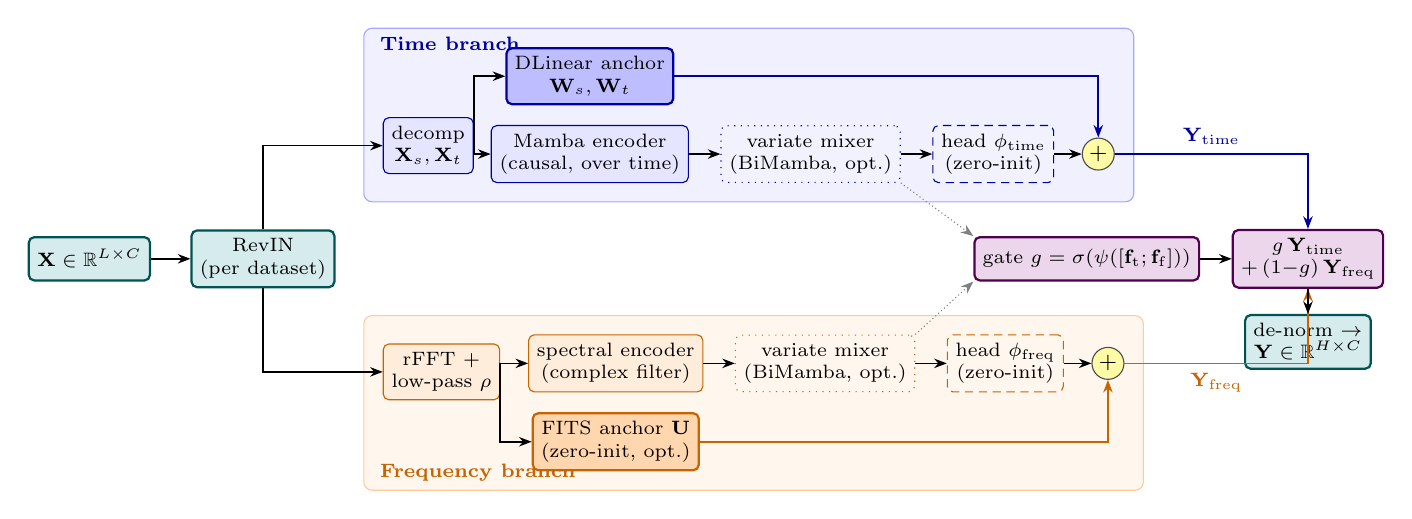
\begin{tikzpicture}[
  font=\scriptsize,
  box/.style={draw, rounded corners=2pt, align=center, inner sep=3pt,
              minimum height=5.5mm, fill=white},
  norm/.style={box, fill=teal!16, draw=teal!65!black, thick},
  tbox/.style={box, fill=blue!10, draw=blue!62!black},
  tanchor/.style={box, fill=blue!26, draw=blue!62!black, thick},
  tzero/.style={box, densely dashed, fill=blue!5, draw=blue!62!black},
  topt/.style={box, dotted, fill=blue!5, draw=blue!62!black},
  fbox/.style={box, fill=orange!14, draw=orange!78!black},
  fanchor/.style={box, fill=orange!32, draw=orange!78!black, thick},
  fzero/.style={box, densely dashed, fill=orange!7, draw=orange!78!black},
  fopt/.style={box, dotted, fill=orange!7, draw=orange!78!black},
  fusebox/.style={box, fill=violet!16, draw=violet!62!black, thick},
  sumc/.style={circle, draw=black!70, inner sep=1pt, fill=yellow!35, font=\footnotesize},
  arr/.style={-{Stealth[length=1.6mm]}, semithick},
  feat/.style={-{Stealth[length=1.6mm]}, densely dotted, gray},
  node distance=3.2mm and 5mm]

% input / normalization
\node[norm] (inp) {$\mathbf{X}\in\mathbb{R}^{L\times C}$};
\node[norm, right=of inp] (revin) {RevIN\\(per dataset)};

% time branch (top row)
\node[tbox, above right=7mm and 6mm of revin] (dec) {decomp\\$\mathbf{X}_s,\mathbf{X}_t$};
\node[tanchor, above right=1.5mm and 4mm of dec] (dlin) {DLinear anchor\\$\mathbf{W}_s,\mathbf{W}_t$};
\node[tbox, below=2.5mm of dlin] (mamba) {Mamba encoder\\(causal, over time)};
\node[topt, right=4mm of mamba] (mixT) {variate mixer\\(BiMamba, opt.)};
\node[tzero, right=4mm of mixT] (headT) {head $\phi_{\mathrm{time}}$\\(zero-init)};
\node[sumc, right=3.5mm of headT] (sumT) {$+$};

% freq branch (bottom row)
\node[fbox, below right=7mm and 6mm of revin] (fft) {rFFT +\\low-pass $\rho$};
\node[fanchor, below right=1.5mm and 4mm of fft] (fits) {FITS anchor $\mathbf{U}$\\(zero-init, opt.)};
\node[fbox, above=2.5mm of fits] (spec) {spectral encoder\\(complex filter)};
\node[fopt, right=4mm of spec] (mixF) {variate mixer\\(BiMamba, opt.)};
\node[fzero, right=4mm of mixF] (headF) {head $\phi_{\mathrm{freq}}$\\(zero-init)};
\node[sumc, right=3.5mm of headF] (sumF) {$+$};

% fusion
\node[fusebox, right=19mm of revin, xshift=62mm] (gate)
  {gate $g=\sigma(\psi([\mathbf{f}_{\mathrm{t}};\mathbf{f}_{\mathrm{f}}]))$};
\node[fusebox, right=4mm of gate] (fuse)
  {$g\,\mathbf{Y}_{\mathrm{time}}$\\$+\,(1{-}g)\,\mathbf{Y}_{\mathrm{freq}}$};
\node[norm, below=3.2mm of fuse] (out) {de-norm $\rightarrow$\\$\mathbf{Y}\in\mathbb{R}^{H\times C}$};

% layered branch panels (drawn behind the nodes)
\begin{scope}[on background layer]
  \node[fill=blue!6, rounded corners=3pt, draw=blue!35, inner sep=2.4mm,
        fit=(dec)(dlin)(mixT)(sumT)] (tpanel) {};
  \node[anchor=north west, font=\scriptsize\bfseries, blue!62!black]
        at (tpanel.north west) {\;Time branch};
  \node[fill=orange!7, rounded corners=3pt, draw=orange!40, inner sep=2.4mm,
        fit=(fft)(fits)(mixF)(sumF)] (fpanel) {};
  \node[anchor=south west, font=\scriptsize\bfseries, orange!78!black]
        at (fpanel.south west) {\;Frequency branch};
\end{scope}

% edges
\draw[arr] (inp) -- (revin);
\draw[arr] (revin.north) |- (dec.west);
\draw[arr] (revin.south) |- (fft.west);
\draw[arr] (dec.east) |- (dlin.west);
\draw[arr] (dec.east) |- (mamba.west);
\draw[arr] (mamba) -- (mixT);
\draw[arr] (mixT) -- (headT);
\draw[arr] (headT) -- (sumT);
\draw[arr, blue!62!black] (dlin.east) -| (sumT.north);
\draw[arr] (fft.east) |- (fits.west);
\draw[arr] (fft.east) |- (spec.west);
\draw[arr] (spec) -- (mixF);
\draw[arr] (mixF) -- (headF);
\draw[arr] (headF) -- (sumF);
\draw[arr, orange!78!black] (fits.east) -| (sumF.south);
\draw[arr, blue!62!black] (sumT.east) -| node[pos=0.25, above]{$\mathbf{Y}_{\mathrm{time}}$} (fuse.north);
\draw[arr, orange!78!black] (sumF.east) -| node[pos=0.25, below]{$\mathbf{Y}_{\mathrm{freq}}$} (fuse.south);
\draw[feat] (mixT.south east) -- (gate.north west);
\draw[feat] (mixF.north east) -- (gate.south west);
\draw[arr] (gate) -- (fuse);
\draw[arr] (fuse) -- (out);
\end{tikzpicture}}
\caption{\model{} overview, color-coded by role: the \textcolor{teal!65!black}{\textbf{normalization}}
wrapper (teal), the \textcolor{blue!62!black}{\textbf{time branch}} (blue),
the \textcolor{orange!78!black}{\textbf{frequency branch}} (orange), and the
\textcolor{violet!62!black}{\textbf{convex-gate fusion}} (violet). In each
branch a solid-filled \emph{linear anchor} runs in parallel with a
zero-initialized nonlinear head (dashed), so at initialization the model
reduces to a linear map of the instance-normalized window. Dotted boxes are
per-dataset switches; dotted grey arrows carry branch features to the gate,
whose convex weight $g$ mixes the two coloured forecast paths
$\mathbf{Y}_{\mathrm{time}}$ and $\mathbf{Y}_{\mathrm{freq}}$.}
\label{fig:arch}
\end{figure}


\subsection{Problem Formulation and Normalization}

Given a look-back window $\mathbf{X} \in \mathbb{R}^{L \times C}$ of $L$
steps and $C$ variates, the task is to predict the next $H$ steps
$\mathbf{Y} \in \mathbb{R}^{H \times C}$. Following RevIN \cite{revin}, we
standardize each window per variate, $\tilde{\mathbf{X}} = (\mathbf{X} -
\boldsymbol{\mu}) / \boldsymbol{\sigma}$, and de-normalize the final
forecast. Instance normalization is treated as a per-dataset switch rather
than a universal default; Sect.~\ref{sec:ablation} shows why.

\subsection{Time Branch: Decomposition, Linear Backbone, Selective Scan}
\label{sec:anchors}

The time branch decomposes $\tilde{\mathbf{X}}$ with a moving average into
trend $\mathbf{X}_t$ and seasonal $\mathbf{X}_s$ components
\cite{autoformer,dlinear} and forecasts with two cooperating paths.

\emph{Linear backbone.} Per-component linear maps project the window
directly to the horizon:
\begin{equation}
\mathbf{Y}_{\mathrm{lin}} = \mathbf{W}_s \mathbf{X}_s +
\mathbf{W}_t \mathbf{X}_t \in \mathbb{R}^{H \times C},
\qquad \mathbf{W}_s, \mathbf{W}_t \in \mathbb{R}^{H \times L},
\end{equation}
i.e., a DLinear-style map \cite{dlinear} (randomly initialized and
trained jointly --- a parameterized pathway, not a fitted DLinear),
shared across variates.

\emph{Selective-scan correction.} The pair $[\mathbf{X}_s; \mathbf{X}_t]$
is embedded per time step and processed channel-independently by a stack
of Mamba layers \cite{mamba}. A Mamba layer discretizes a state-space
system with input-dependent parameters
$(\boldsymbol{\Delta}, \mathbf{B}, \mathbf{C})$:
\begin{equation}
\mathbf{h}_k = e^{\boldsymbol{\Delta}_k \mathbf{A}}\,\mathbf{h}_{k-1} +
\boldsymbol{\Delta}_k \mathbf{B}_k\, u_k, \qquad
y_k = \mathbf{C}_k^{\top} \mathbf{h}_k + D\, u_k ,
\label{eq:ssm}
\end{equation}
scanned causally over the $L$ steps and applied independently to each of
the $d_{\mathrm{in}}$ feature dimensions: per dimension, the state is
$\mathbf{h}_k \in \mathbb{R}^{N}$, $\mathbf{A} \in \mathbb{R}^{N}$ is
diagonal, the input $u_k$ is scalar, and
$(\boldsymbol{\Delta}_k \in \mathbb{R},\; \mathbf{B}_k, \mathbf{C}_k \in
\mathbb{R}^{N})$ are produced from $u$ by learned linear maps
\cite{mamba}. The last state, summed with a
whole-window linear embedding $\mathbf{W}_e \tilde{\mathbf{x}}^{(c)}$
(one per variate, as in \cite{smamba}), forms the branch feature
$\mathbf{f}_{\mathrm{time}} \in \mathbb{R}^{C \times d}$. A head
$\phi_{\mathrm{time}}$ maps features to a horizon correction:
\begin{equation}
\mathbf{Y}_{\mathrm{time}} = \mathbf{Y}_{\mathrm{lin}} +
\phi_{\mathrm{time}}(\mathbf{f}_{\mathrm{time}}), \qquad
\phi_{\mathrm{time}} \equiv \mathbf{0} \text{ at init.}
\label{eq:timezero}
\end{equation}
Because $\phi_{\mathrm{time}}$ is zero-initialized, the branch's output
at initialization equals its (randomly initialized) DLinear-style
backbone; the SSM learns only what the linear map cannot express. We compute the recurrence of Eq.~\eqref{eq:ssm} in fp32 even
under mixed-precision training: the exponential and the $L$-step state
accumulation overflow in half precision, which silently destroys training
(observed as NaN validation losses that exhaust early-stopping patience).

\subsection{Frequency Branch: Spectral Filtering and a FITS Anchor}
\label{sec:freq}

The frequency branch applies the real FFT along time,
$\mathbf{Z} = \mathrm{rFFT}(\tilde{\mathbf{X}}) \in
\mathbb{C}^{C \times F}$, $F = \lfloor L/2 \rfloor + 1$, optionally
low-passed by zeroing the top fraction $\rho$ of bins.

\emph{Spectral encoder.} A learnable complex linear filter
$\mathbf{W} = \mathbf{W}_r + i\mathbf{W}_i$ densely mixes bins,
$\mathbf{Z}' = \mathbf{Z}\mathbf{W}^{\top} \in \mathbb{C}^{C \times F}$
with $\mathbf{W} \in \mathbb{C}^{F \times F}$ acting along the frequency
axis, realized with two real matrices;
a bidirectional Mamba over the bin sequence is available as an
input-dependent alternative. The (real, imaginary) parts are projected to
the branch feature $\mathbf{f}_{\mathrm{freq}} \in \mathbb{R}^{C \times d}$
and a head $\phi_{\mathrm{freq}}$ produces the spectral forecast.

\emph{FITS anchor (optional, per dataset).} Mirroring the time branch, a
complex linear map
$\mathbf{U} \in \mathbb{C}^{F' \times F}$ with
$F' = \lfloor (L{+}H)/2 \rfloor + 1$, applied along the frequency axis
($\mathbf{Z}\mathbf{U}^{\top} \in \mathbb{C}^{C \times F'}$), maps the
(low-passed) window spectrum to that of a length-$(L{+}H)$ series, whose inverse transform's last $H$
samples are the branch's linear spectral forecast:
\begin{equation}
\mathbf{Y}_{\mathrm{freq}} =
\underbrace{\mathrm{irFFT}_{L+H}(\mathbf{Z}\mathbf{U}^{\top})[\,L{:}\,]}_{\text{linear-in-frequency}}
\; + \; \phi_{\mathrm{freq}}(\mathbf{f}_{\mathrm{freq}}),
\qquad \mathbf{U}, \phi_{\mathrm{freq}} \equiv \mathbf{0} \text{ at init.}
\label{eq:fits}
\end{equation}
This pathway \emph{parameterizes} the FITS \cite{fits} family --- any
linear-in-frequency forecaster of the low-passed spectrum is reachable ---
but, unlike FITS itself, $\mathbf{U}$ is \emph{zero-initialized}, so the
frequency branch is silent at initialization rather than a functioning
spectral predictor. This is deliberate: the frequency grids of a length-$L$
and a length-$(L{+}H)$ window do not align (harmonic $k$ of the input maps
to the non-integer index $k(L{+}H)/L$ of the output), so no canonical
identity or interpolation initialization exists; a randomly initialized
$\mathbf{U}$ would inject noise into the fused forecast during the
highest-learning-rate epochs. Zero initialization instead lets the gate
lean on the time anchor until $\mathbf{U}$ is learned jointly with the
rest of the model. Consequently, the precise initialization claim is: the
time branch coincides with a (randomly initialized) DLinear, the frequency
branch outputs zero, and the fusion gate is the constant $g_0$
(Sect.~\ref{sec:fusion}), so in the instance-normalized space the
end-to-end map is the linear function $g_0 \cdot
\mathbf{Y}_{\mathrm{lin}}$. Composed with RevIN --- whose window
statistics are themselves a nonlinear function of the input --- the model
at initialization is a randomly initialized linear map wrapped in
instance normalization, exactly the structure of RLinear-class models
\cite{rlinear,revin}; it is linear in the normalized window, not in the
raw input, and it is linear by construction, not a fitted linear model. The anchor is enabled per
dataset (ETTh1, ETTh2, and Weather; Table~\ref{tab:hparams}); where it is
disabled, the frequency branch remains fully active through its spectral
encoder and head but carries no explicit linear pathway, so the
linear-anchoring property then rests on the time branch alone.

\subsection{Cross-Channel Mixing over Variates}
\label{sec:mixer}

Channel independence is a strong baseline \cite{patchtst,dlinear} but
leaves accuracy on the table when variates are strongly coupled
\cite{itransformer,smamba}. Inside each branch, before its head, we
optionally run $M$ layers of \emph{bidirectional} Mamba over the variate
dimension --- treating the $C$ per-channel features as a sequence ---
followed by a position-wise feed-forward block. Bidirectionality is
essential: channel order carries no causal direction, so each layer runs
forward and reversed scans and sums them in one residual stream. The mixer
is a per-dataset choice: $M{=}2$ at width 512 on electricity/traffic
(where it is the single most load-bearing component;
Sect.~\ref{sec:ablation}), $M{=}2$ at width 256 on weather, $M{=}1$ on
solar, and $M{=}0$ on the 7--8-channel ETT and exchange datasets, where it
triples parameters without adding signal.

\subsection{Forecast-Level Convex Fusion}
\label{sec:fusion}

Each branch emits a forecast and a feature. The model output is a gated
convex combination
\begin{equation}
\mathbf{Y} = g \odot \mathbf{Y}_{\mathrm{time}} + (1 - g) \odot
\mathbf{Y}_{\mathrm{freq}}, \qquad
g = \sigma\!\big(\psi([\mathbf{f}_{\mathrm{time}};
\mathbf{f}_{\mathrm{freq}}])\big) \in (0,1)^{C\times 1},
\label{eq:fusion}
\end{equation}
with $\psi$ applied row-wise (per variate), followed by RevIN
de-normalization. Since $\mathbf{Y}$ lies elementwise between the branch
forecasts, both domains retain an explicit prediction path, and the gate
value reports each branch's convex mixing weight --- a lightweight proxy
for its contribution, not a causal attribution. The constraint is
structural, not behavioral: $g$ is a sigmoid and can saturate near 0 or 1,
so one branch may contribute very little --- by design, as the ablations
show the useful domain is dataset-dependent. $\psi$ is zero-initialized
with bias $2.2$, so training starts at $g \approx 0.9$: the time branch is
linear at initialization while the frequency branch is silent, and an even
$0.5/0.5$ mix would waste the highest-learning-rate epochs on noise.

\subsection{Training}

We minimize MSE with AdamW under a halving schedule
($\eta_e = \eta_0 \cdot 2^{-(e-1)}$), which concentrates learning in the
first epochs and suppresses the late-epoch overfitting that cosine
schedules invite on small benchmarks. All runs use 10 epochs; early
stopping monitors validation loss with the best checkpoint restored.

\section{Experiments}
\label{sec:experiments}

\subsection{Setup}
\label{sec:setup}

\paragraph{Datasets and protocol.} We evaluate on nine standard benchmarks
(Table~\ref{tab:datasets}) under the unified protocol of
\cite{itransformer,smamba}: look-back $L{=}96$ for all datasets and
horizons $H \in \{96, 192, 336, 720\}$; ETT uses the canonical 12/4/4-month
border split (the file tail beyond month 20 is unused), the others
chronological 0.7/0.1/0.2 splits; variates are standardized by training-set
statistics; metrics are MSE and MAE on the standardized test set.

\begin{table}[t]
\centering
\caption{Benchmark datasets and where \model{} places its capacity.}
\label{tab:datasets}
\begin{tabular}{@{}lrrlll@{}}
\toprule
Dataset & Variates & Steps & Granularity & Variate mixer & Params \\
\midrule
ETTh1/ETTh2 & 7 & 17{,}420 & 1 hour & off & 0.25M \\
ETTm1/ETTm2 & 7 & 69{,}680 & 15 min & off & 0.24--0.36M \\
Weather & 21 & 52{,}696 & 10 min & $M{=}2$, $d{=}256$ & 5.8M \\
Solar-Energy & 137 & 52{,}560 & 10 min & $M{=}1$, $d{=}128$ & 0.96M \\
Electricity & 321 & 26{,}304 & 1 hour & $M{=}2$, $d{=}512$ & 19.7M \\
Traffic & 862 & 17{,}544 & 1 hour & $M{=}2$, $d{=}512$ & 19.7M \\
Exchange & 8 & 7{,}588 & 1 day & off & 0.09M \\
\bottomrule
\end{tabular}
\end{table}

\paragraph{Baselines.} We compare against the strongest published results
under the same protocol: the state-space forecaster S-Mamba \cite{smamba},
iTransformer \cite{itransformer}, PatchTST \cite{patchtst}, DLinear
\cite{dlinear}, and TimesNet \cite{timesnet}. Baseline numbers are quoted
from \cite{smamba} rather than reproduced: the evaluation protocol
(look-back, splits, standardization, metrics) is identical, but training
pipelines, seeds, and implementations differ across works, so
sub-noise-floor gaps to quoted numbers should be read with caution. We
flag every such case in the text, and re-running all baselines within one
unified training framework is planned for the camera-ready appendix.

\subsubsection{Implementation and Reproducibility.}
\label{sec:repro}
All experiments use PyTorch 2.11 (CUDA 13.0) on a single NVIDIA RTX 5090
(32\,GB). Optimization is AdamW with gradient clipping at $5.0$, 10 epochs
with the learning rate halved after every epoch, early stopping on
validation loss with the best checkpoint restored, and mixed precision
with the selective scan forced to fp32 (Sect.~\ref{sec:anchors}). The
decomposition kernel is 25; Mamba blocks use expansion 2 and depthwise
convolution width 4 throughout. Table~\ref{tab:hparams} lists all
per-dataset settings; complete configuration files and the ablation
harness ship with the code. All main results (Tables~\ref{tab:main} and
\ref{tab:horizons}) are means over \emph{three seeds} (2024--2026);
Table~\ref{tab:horizons} reports the per-entry standard deviations, whose
maximum across all 36 dataset--horizon entries is $0.005$ MSE (Solar,
$H{=}720$) with a typical value of $0.001$--$0.003$. \paragraph{Statistical methodology.} We compare at two levels.
\emph{Within our framework} (ablations), every variant shares seeds with
the reference, so we report \emph{paired} per-seed differences with
$t$-based 95\% CIs ($n{=}3$) and treat a component as supported only when
its CI excludes zero. \emph{Against quoted baselines}, pairing is
impossible, so we use a conservative unpaired tie threshold of $0.005$
MSE. Our in-framework DLinear re-run shows why: through the identical
pipeline on ETTh1 (three seeds) it averages $0.462$/$0.456$ MSE/MAE versus
its quoted $0.456$/$0.452$ --- a $+0.006$ implementation gap, the order of
several margins in Table~\ref{tab:main}. Cross-paper comparisons therefore
cannot support sub-$0.01$ distinctions; re-running S-Mamba, iTransformer,
and PatchTST here is the planned resolution. \model{}'s margin over the
in-framework DLinear ($0.439$ vs.\ $0.462$) is, by contrast, a
same-pipeline comparison, roughly six times the largest observed std.

\begin{table}[t]
\centering
\caption{Per-dataset hyperparameters. $d$: model width; time enc.:
time-branch encoder (Mamba layers in parentheses); $M$: variate-mixer
layers; $N$: SSM state size; $\rho$: spectral low-pass fraction
(Sect.~\ref{sec:freq}); FITS: the \emph{optional} spectral linear anchor of Eq.~\eqref{eq:fits}
--- when ``no'', the frequency branch remains fully active (rFFT, spectral
encoder, forecast head) but carries no explicit linear pathway; IN:
instance normalization (RevIN); do.: dropout; B: batch size; wd: weight
decay. $^{\dagger}$Solar adopts IN~=~no from the ablation finding
(Sect.~\ref{sec:ablation}); its main results were re-measured under this
configuration across all horizons and seeds.}
\label{tab:hparams}
\scriptsize
\setlength{\tabcolsep}{3.2pt}
\begin{tabular}{@{}lcccccccccc@{}}
\toprule
Dataset & $d$ & time enc. & $M$ & $N$ & $\rho$ & FITS & IN & lr & B & do./wd \\
\midrule
ETTh1 & 128 & Mamba (1) & 0 & 16 & 0.4 & yes & yes & $5{\cdot}10^{-4}$ & 32 & 0.2/$10^{-4}$ \\
ETTh2 & 128 & Mamba (1) & 0 & 16 & 0.3 & yes & yes & $5{\cdot}10^{-4}$ & 32 & 0.3/$5{\cdot}10^{-4}$ \\
ETTm1 & 128 & Mamba (2) & 0 & 16 & 0 & no & yes & $10^{-4}$ & 32 & 0.1/$10^{-4}$ \\
ETTm2 & 128 & Mamba (1) & 0 & 16 & 0.2 & no & yes & $10^{-4}$ & 32 & 0.2/$2{\cdot}10^{-4}$ \\
Weather & 256 & Mamba (2) & 2 & 16 & 0 & yes & yes & $2{\cdot}10^{-4}$ & 32 & 0.1/$10^{-4}$ \\
Solar & 128 & Mamba (2) & 1 & 16 & 0 & no & no$^{\dagger}$ & $5{\cdot}10^{-4}$ & 16 & 0.1/$10^{-4}$ \\
Electricity & 512 & MLP & 2 & 32 & 0 & no & yes & $5{\cdot}10^{-4}$ & 16 & 0.1/$10^{-4}$ \\
Traffic & 512 & MLP & 2 & 32 & 0 & no & yes & $10^{-3}$ & 16 & 0.1/$10^{-4}$ \\
Exchange & 64 & Mamba (1) & 0 & 8 & 0.5 & no & yes & $10^{-4}$ & 32 & 0.3/$5{\cdot}10^{-4}$ \\
\bottomrule
\end{tabular}
\end{table}

\subsection{Main Results}

\begin{table}[t]
\centering
\caption{Long-term forecasting results averaged over horizons
$H \in \{96,192,336,720\}$ with look-back $L{=}96$ (MSE/MAE; lower is
better). \model{} entries are means over three seeds
(Table~\ref{tab:horizons} reports per-horizon std). Baselines quoted from
\cite{smamba}. \textbf{Bold} marks the
best result \emph{and} every result within the run-to-run noise floor
($<0.005$, Sect.~\ref{sec:repro}) of it, treated as tied best;
\underline{underline} marks the next-best result.}
\label{tab:main}
\scriptsize
\setlength{\tabcolsep}{2.6pt}
\begin{tabular}{@{}lcccccc@{}}
\toprule
Dataset & \model{} (ours) & S-Mamba & iTransformer & PatchTST & DLinear & TimesNet \\
\midrule
ETTh1 & \best{0.439}/\best{0.434} & 0.455/0.450 & \second{0.454}/\second{0.447} & 0.469/0.454 & 0.456/0.452 & 0.458/0.450 \\
ETTh2 & \best{0.374}/\best{0.401} & \second{0.381}/\best{0.405} & 0.383/\second{0.407} & 0.387/\second{0.407} & 0.559/0.515 & 0.414/0.427 \\
ETTm1 & \best{0.386}/\best{0.398} & \second{0.398}/\second{0.405} & 0.407/0.410 & \best{0.387}/\best{0.400} & 0.403/0.407 & 0.400/0.406 \\
ETTm2 & \best{0.280}/\best{0.325} & \second{0.288}/\second{0.332} & \second{0.288}/\second{0.332} & \best{0.281}/\best{0.326} & 0.350/0.401 & 0.291/0.333 \\
Weather & \best{0.248}/\best{0.276} & \best{0.251}/\best{0.276} & \second{0.258}/\best{0.278} & 0.259/\second{0.281} & 0.265/0.317 & 0.259/0.287 \\
Electricity & \best{0.168}/\best{0.263} & \best{0.170}/\best{0.265} & \second{0.178}/\second{0.270} & 0.205/0.290 & 0.212/0.300 & 0.192/0.295 \\
Traffic & 0.438/\second{0.281} & \best{0.414}/\best{0.276} & \second{0.428}/0.282 & 0.481/0.304 & 0.625/0.383 & 0.620/0.336 \\
Exchange & 0.363/\best{0.405} & 0.367/\second{0.408} & \second{0.360}/\best{0.403} & 0.367/\best{0.404} & \best{0.354}/0.414 & 0.416/0.443 \\
Solar & \best{0.199}/\best{0.260} & 0.240/\second{0.273} & \second{0.233}/\best{0.262} & 0.270/0.307 & 0.330/0.401 & 0.301/0.319 \\
\bottomrule
\end{tabular}
\end{table}

\begin{table}[t]
\centering
\caption{\model{} per-horizon results (mean $\pm$ std over three
seeds), look-back $L{=}96$.}
\label{tab:horizons}
\scriptsize
\setlength{\tabcolsep}{3.0pt}
\begin{tabular}{@{}llccccc@{}}
\toprule
Dataset & & $H{=}96$ & $H{=}192$ & $H{=}336$ & $H{=}720$ & Avg \\
\midrule
ETTh1 & MSE & $0.380{\scriptstyle\pm.001}$ & $0.431{\scriptstyle\pm.002}$ & $0.474{\scriptstyle\pm.004}$ & $0.470{\scriptstyle\pm.003}$ & 0.439 \\
 & MAE & $0.396{\scriptstyle\pm.001}$ & $0.424{\scriptstyle\pm.001}$ & $0.447{\scriptstyle\pm.003}$ & $0.468{\scriptstyle\pm.001}$ & 0.434 \\
ETTh2 & MSE & $0.293{\scriptstyle\pm.001}$ & $0.368{\scriptstyle\pm.003}$ & $0.414{\scriptstyle\pm.001}$ & $0.421{\scriptstyle\pm.001}$ & 0.374 \\
 & MAE & $0.344{\scriptstyle\pm.002}$ & $0.391{\scriptstyle\pm.000}$ & $0.426{\scriptstyle\pm.000}$ & $0.441{\scriptstyle\pm.001}$ & 0.401 \\
ETTm1 & MSE & $0.320{\scriptstyle\pm.001}$ & $0.366{\scriptstyle\pm.002}$ & $0.398{\scriptstyle\pm.001}$ & $0.462{\scriptstyle\pm.001}$ & 0.386 \\
 & MAE & $0.359{\scriptstyle\pm.001}$ & $0.384{\scriptstyle\pm.001}$ & $0.406{\scriptstyle\pm.001}$ & $0.443{\scriptstyle\pm.001}$ & 0.398 \\
ETTm2 & MSE & $0.177{\scriptstyle\pm.000}$ & $0.242{\scriptstyle\pm.002}$ & $0.302{\scriptstyle\pm.000}$ & $0.401{\scriptstyle\pm.003}$ & 0.280 \\
 & MAE & $0.260{\scriptstyle\pm.001}$ & $0.303{\scriptstyle\pm.001}$ & $0.340{\scriptstyle\pm.000}$ & $0.398{\scriptstyle\pm.002}$ & 0.325 \\
Weather & MSE & $0.162{\scriptstyle\pm.000}$ & $0.212{\scriptstyle\pm.000}$ & $0.269{\scriptstyle\pm.001}$ & $0.352{\scriptstyle\pm.003}$ & 0.248 \\
 & MAE & $0.207{\scriptstyle\pm.001}$ & $0.255{\scriptstyle\pm.000}$ & $0.295{\scriptstyle\pm.002}$ & $0.349{\scriptstyle\pm.002}$ & 0.276 \\
Electricity & MSE & $0.140{\scriptstyle\pm.000}$ & $0.157{\scriptstyle\pm.001}$ & $0.174{\scriptstyle\pm.001}$ & $0.200{\scriptstyle\pm.004}$ & 0.168 \\
 & MAE & $0.235{\scriptstyle\pm.000}$ & $0.252{\scriptstyle\pm.001}$ & $0.271{\scriptstyle\pm.001}$ & $0.296{\scriptstyle\pm.004}$ & 0.263 \\
Traffic & MSE & $0.402{\scriptstyle\pm.002}$ & $0.424{\scriptstyle\pm.001}$ & $0.441{\scriptstyle\pm.001}$ & $0.485{\scriptstyle\pm.003}$ & 0.438 \\
 & MAE & $0.266{\scriptstyle\pm.001}$ & $0.275{\scriptstyle\pm.001}$ & $0.283{\scriptstyle\pm.000}$ & $0.301{\scriptstyle\pm.000}$ & 0.281 \\
Exchange & MSE & $0.086{\scriptstyle\pm.000}$ & $0.179{\scriptstyle\pm.001}$ & $0.330{\scriptstyle\pm.002}$ & $0.857{\scriptstyle\pm.001}$ & 0.363 \\
 & MAE & $0.205{\scriptstyle\pm.000}$ & $0.301{\scriptstyle\pm.000}$ & $0.416{\scriptstyle\pm.002}$ & $0.699{\scriptstyle\pm.000}$ & 0.405 \\
Solar & MSE & $0.180{\scriptstyle\pm.004}$ & $0.195{\scriptstyle\pm.005}$ & $0.207{\scriptstyle\pm.001}$ & $0.212{\scriptstyle\pm.005}$ & 0.199 \\
 & MAE & $0.237{\scriptstyle\pm.003}$ & $0.259{\scriptstyle\pm.003}$ & $0.270{\scriptstyle\pm.001}$ & $0.274{\scriptstyle\pm.005}$ & 0.260 \\
\bottomrule
\end{tabular}
\end{table}

Table~\ref{tab:main} summarizes averages over the four horizons;
Table~\ref{tab:horizons} reports \model{} per horizon with per-entry
standard deviations. Applying the noise-floor tie rule consistently,
\model{} reports the lowest average MSE on seven of the nine datasets.
The margin over the best baseline is clear on Solar ($0.199$ vs.\
iTransformer's $0.233$; $-17\%$ vs.\ S-Mamba, roughly seven times the
largest observed std --- measured with the instance-normalization-free
configuration from Sect.~\ref{sec:ablation}), on ETTh1 ($-0.015$), and
on ETTh2 ($-0.007$); on ETTm1/ETTm2 the margin over S-Mamba is clear
($-0.012$/$-0.008$) but the gap to PatchTST is $0.001$ --- a tie; on
Weather ($-0.003$) and Electricity ($-0.002$) the lead over S-Mamba is
below the floor and the methods should be read as tied. \model{} remains
competitive on Exchange --- a near random-walk dataset where all methods
cluster within $0.013$ MSE and plain DLinear is best, $0.009$ ahead of
\model{} --- and lags S-Mamba on Traffic by $+0.024$ MSE. We
\emph{hypothesize} the traffic deficit stems from the weekly cycle
exceeding the protocol look-back; this is not yet experimentally
verified, and Sect.~\ref{sec:conclusion} lists the experiments that
would test it. All comparisons are relative to results \emph{reported}
in \cite{smamba} under the same protocol (Sect.~\ref{sec:setup}), so we phrase our
overall claim conservatively: \model{} is competitive with results
reported under the same protocol. Its largest margin is on Solar, driven
by per-dataset normalization; the next largest are on the small ETT
datasets, where the linear anchors and deliberate capacity restraint
matter most --- there \model{} uses roughly $0.25$M parameters, two
orders of magnitude fewer than variate-attention models configured for
those datasets.

\subsection{Component Ablations}
\label{sec:ablation}

We release an ablation harness in which every variant flips exactly one
switch of a dataset's full configuration, holding the split, schedule,
seeds, and all other hyperparameters fixed. We report its complete output
on three datasets under their \emph{final released configurations}, three
seeds each and all at $H{=}96$: ETTh1 and Solar-Energy
(Table~\ref{tab:ablation}) and Weather
(Table~\ref{tab:ablation_weather}), analyzed with the paired methodology
of Sect.~\ref{sec:repro}. Two internal consistency checks pass: the Solar
``full'' row reproduces the main-table Solar $H{=}96$ entry exactly
($0.180{\scriptstyle\pm.004}$), and Solar's w/o-instance-norm variant
coincides with its full configuration (which already disables RevIN), so
that cell is omitted.

\begin{table}[t]
\centering
\caption{Component ablations on ETTh1 and Solar-Energy ($H{=}96$, three
seeds, final configurations): paired per-seed $\Delta$MSE to the full
model with $t$-based 95\% CIs; $^{*}$\,CI excludes zero. The FITS anchor
is enabled on ETTh1 (hence \emph{removed}) and disabled on Solar (hence
\emph{added}); the variate mixer is off on ETTh1 (\emph{added}) and on
for Solar (\emph{removed}).}
\label{tab:ablation}
\scriptsize
\setlength{\tabcolsep}{3pt}
\begin{tabular}{@{}lcc@{}}
\toprule
Variant & ETTh1: $\Delta$ [95\% CI] & Solar: $\Delta$ [95\% CI] \\
\midrule
full (reference MSE) & $0.3802{\scriptstyle\pm.001}$ & $0.1802{\scriptstyle\pm.004}$ \\
\;\;time branch only (freq removed) & $+0.0034$ $[-0.009,+0.016]$ & $+0.0114$ $[+0.001,+0.021]$$^{*}$ \\
\;\;freq branch only (time removed) & $-0.0007$ $[-0.004,+0.003]$ & $+0.0051$ $[-0.013,+0.023]$ \\
\;\;sum fusion & $-0.0026$ $[-0.007,+0.002]$ & $+0.0066$ $[-0.005,+0.018]$ \\
\;\;w/o instance norm & $+0.0061$ $[-0.001,+0.013]$ & --- \\
\;\;w/o linear backbone & $-0.0031$ $[-0.009,+0.003]$ & $+0.0081$ $[-0.019,+0.035]$ \\
\;\;random init (vs.\ zero-init) & $-0.0012$ $[-0.005,+0.002]$ & $-0.0046$ $[-0.022,+0.013]$ \\
\;\;FITS anchor removed / added & $+0.0042$ $[-0.018,+0.026]$ & $+0.0088$ $[-0.002,+0.019]$ \\
\;\;variate mixer added / removed & $+0.0077$ $[+0.004,+0.012]$$^{*}$ & $+0.0119$ $[-0.010,+0.034]$ \\
\;\;Mamba$\rightarrow$MLP over time & $-0.0022$ $[-0.007,+0.003]$ & $+0.0089$ $[-0.002,+0.020]$ \\
\;\;freq Mamba encoder & $-0.0024$ $[-0.011,+0.006]$ & $-0.0117$ $[-0.044,+0.020]$ \\
\bottomrule
\end{tabular}
\end{table}

\paragraph{Dual-domain evidence.} The decisive result is on Solar:
removing the frequency branch degrades MSE by $+0.0114$ with a CI
excluding zero --- the first statistically supported frequency-branch
contribution in our studies. On ETTh1 and Weather, by contrast, both
single-branch variants lie within their CIs; on ETTh1 the frequency
branch \emph{alone} even matches the full model ($-0.0007$), i.e., the
two branches are largely redundant there. The dual-domain claim our data
supports is therefore conditional: the frequency path contributes
measurably on Solar and is redundant, though not harmful, on the other
two ablated datasets.

\paragraph{Capacity placement, validated in both directions.} Adding the
variate mixer on ETTh1 \emph{hurts} ($+0.0077$, CI $[+0.004,+0.012]$),
while removing it on Weather also hurts ($+0.0104$, $[+0.004,+0.017]$)
--- significant paired evidence on both sides of the placement decision.
Instance normalization shows the same two-sided pattern: removing it
hurts Weather ($+0.0161$, $[+0.005,+0.027]$), while \emph{disabling} it
on Solar improved the re-measured main results from $0.228$ to $0.199$
average MSE (a legacy single-seed probe on the pre-final Solar
configuration first surfaced this as $-0.016$ MSE at $H{=}96$).

\paragraph{Zero initialization: a null result.} The controlled
random-initialization comparison --- the harness switch introduced
precisely for this test --- finds no significant accuracy difference on
either dataset ($-0.0012$ on ETTh1, $-0.0046$ on Solar; both CIs include
zero). We therefore make no accuracy claim for zero initialization: its
value in this framework is the interpretable linear start of
Sect.~\ref{sec:anchors}, and stability-oriented analyses (convergence
curves, failure rates, correction magnitudes) remain future work.

\paragraph{Weaker components.} The DLinear backbone is not individually
significant in any paired study (point estimates $+0.008$ on Solar,
$+0.001$ on Weather, $-0.003$ on ETTh1, where the FITS pathway can
substitute for it), and the learned gate versus plain averaging is
within CIs everywhere. On Weather (Table~\ref{tab:ablation_weather}),
exactly three components survive the paired test: instance normalization
($+0.0161$), the variate mixer ($+0.0104$), and the temporal Mamba
($+0.0027$, $[+0.0020,+0.0034]$, positive on all three seeds); every
other variant's CI includes zero. Across the three studies the recurring
pattern is that component value is dataset-dependent --- in \emph{both}
directions for the mixer and normalization --- which is the argument for
shipping components as per-dataset switches rather than universal
defaults.

\begin{table}[t]
\centering
\caption{Component ablation on Weather ($H{=}96$; MSE mean $\pm$ std over
three seeds). $\Delta$ is the \emph{paired} per-seed difference to the
full model with a $t$-based 95\% confidence interval ($n{=}3$);
$^{*}$\,CI excludes zero.}
\label{tab:ablation_weather}
\scriptsize
\setlength{\tabcolsep}{3pt}
\begin{tabular}{@{}lccl@{}}
\toprule
Variant & MSE & paired $\Delta$ [95\% CI] & Component isolated \\
\midrule
full & $0.1620{\scriptstyle\pm.0003}$ & --- & reference \\
\;\;w/o instance norm & $0.1781{\scriptstyle\pm.0035}$ & $+0.0161$ $[+0.0053,+0.0269]$$^{*}$ & RevIN \\
\;\;w/o channel mixer & $0.1724{\scriptstyle\pm.0021}$ & $+0.0104$ $[+0.0037,+0.0172]$$^{*}$ & cross-variate Mamba mixing \\
\;\;Mamba$\rightarrow$MLP over time & $0.1647{\scriptstyle\pm.0005}$ & $+0.0027$ $[+0.0020,+0.0034]$$^{*}$ & selective scan (time) \\
\;\;w/o linear backbone & $0.1631{\scriptstyle\pm.0006}$ & $+0.0011$ $[-0.0014,+0.0036]$ & DLinear anchor (time) \\
\;\;time branch only & $0.1628{\scriptstyle\pm.0011}$ & $+0.0007$ $[-0.0020,+0.0035]$ & frequency branch removed \\
\;\;w/o FITS anchor & $0.1627{\scriptstyle\pm.0016}$ & $+0.0007$ $[-0.0041,+0.0055]$ & spectral linear anchor \\
\;\;freq branch only & $0.1626{\scriptstyle\pm.0014}$ & $+0.0006$ $[-0.0040,+0.0052]$ & time branch removed \\
\;\;freq Mamba encoder & $0.1626{\scriptstyle\pm.0016}$ & $+0.0006$ $[-0.0044,+0.0055]$ & spectral encoder type \\
\;\;sum fusion & $0.1622{\scriptstyle\pm.0007}$ & $+0.0001$ $[-0.0020,+0.0023]$ & learned gate $\rightarrow$ average \\
\bottomrule
\end{tabular}
\end{table}

\paragraph{Normalization is a per-dataset decision.} The same probe that
revealed RevIN \emph{hurting} solar ($-0.016$ MSE when removed) shows the
opposite on traffic: removing it degrades traffic from $0.405$ to $0.505$
MSE at $H{=}96$. The datasets look alike --- both bounded and strongly
periodic --- but solar's night zeros are \emph{periodic structure} (window
statistics then mostly encode the night fraction, and de-normalization
amplifies errors by an unstable standard deviation), whereas traffic
windows carry genuine distribution shift (weekday/weekend composition,
per-sensor levels) that normalization absorbs. We therefore ship
normalization as a verified per-dataset switch and caution against
transferring its conclusions across datasets.

\paragraph{Negative results that shaped the design.} Deepening the traffic
variate mixer from two to four layers ($19.7 \rightarrow 37.9$M
parameters) gave no accuracy gain, so the release keeps two layers.
Enabling the mixer on ETT (7 channels, $8.4$K training windows) instead
tripled parameters and \emph{caused} premature early stopping through
immediate overfitting; the released ETT configurations disable it.

\begin{figure}[t]
\centering
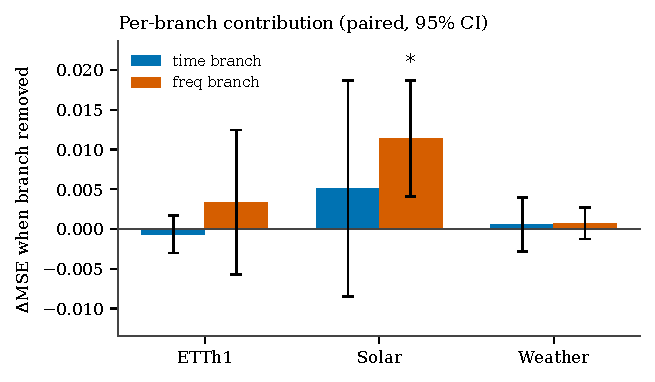
\includegraphics[width=\textwidth]{fig_evidence.pdf}
\caption{Dual-domain evidence. \textbf{(a)}~The learned fusion gate on
ETTh1: the mean convex weight $\bar g_c$ assigned to the \emph{time} branch
for each variate over the test set. Initialized time-heavy at
$g_0{\approx}0.9$ (dashed), the trained gate redistributes weight toward
the frequency branch (below the equal-mix line, dotted), matching the
ETTh1 ablation in which the frequency branch alone reproduces the full
model. \textbf{(b)}~Per-branch contribution: the paired increase in MSE
($H{=}96$, three seeds) when each branch is removed --- freq contribution
$=$ time-only $-$ full, time contribution $=$ freq-only $-$ full --- with
$t$-based 95\% CIs; $^{*}$\,marks a CI clearing zero. Only Solar's
frequency branch is individually significant; on ETTh1 and Weather the
branches are mutually redundant. This is the visual form of our
conditional dual-domain claim: the two domains are complementary on some
datasets and interchangeable on others.}
\label{fig:evidence}
\end{figure}

\subsection{Analysis}

\paragraph{Where each domain wins.} On solar the branch-only ablations
(Table~\ref{tab:ablation}, Fig.~\ref{fig:evidence}b) show both domains
contribute but the time view carries more (removing it costs $+0.012$ MSE
vs.\ $+0.002$ for the frequency branch) --- consistent with the look-back
hiding part of the periodic structure (the 10-minute daily cycle spans
144 samples ${>}\,L{=}96$; likewise weather's daily and traffic's weekly
cycles). Beyond ablations, the fusion gate (Eq.~\eqref{eq:fusion}) exposes
per-sample convex weights --- a proxy for, not a causal measure of, branch
contributions. Figure~\ref{fig:evidence}a reads them on a trained ETTh1
model: initialized at $g_0{\approx}0.9$, the gate settles below equal mix,
shifting weight toward the frequency branch that the ablation certifies as
sufficient. Gate and ablation agree, though only the ablation is causal;
a systematic gate study is left for the extended version.

\paragraph{Efficiency profile.} To make the engineering profile concrete
without tying it to specific hardware, Table~\ref{tab:efficiency} reports
three hardware-independent measurements per dataset: trainable parameters,
multiply--accumulates (MACs) for one forecast, and the forward activation
footprint. Two properties stand out. Parameter count is governed by model
\emph{width}, not channel count --- electricity and traffic share the same
$19.7$M despite an order-of-magnitude gap in variates --- so model size is
decoupled from data dimensionality. Compute and activation memory, by
contrast, scale with the channel count through the bidirectional variate
mixer, which scans $C$ tokens: traffic ($862$ channels) costs $60$\,GMACs
per forecast against electricity's $22$\,GMACs at equal width. The small
ETT and exchange configurations sit two orders of magnitude below, at
$0.02$--$0.08$\,GMACs and under $5$\,MB, which makes the deliberate
capacity restraint on those datasets (Sect.~\ref{sec:mixer}) cheap as well
as accurate. These are properties of the model and input shapes, not
wall-clock figures; a throughput and peak GPU-memory comparison against
S-Mamba, iTransformer, and PatchTST under identical hardware is left for
the extended version.

\begin{table}[t]
\centering
\caption{Engineering profile of \model{} per dataset (look-back 96,
horizon 96, batch~1). GMACs: multiply--accumulates per forecast
(\texttt{Linear} $+$ \texttt{Conv1d} $+$ the selective-scan recurrence);
act.\ mem.: forward activation footprint (fp32). All three columns are
hardware-independent; wall-clock throughput on the RTX~5090 is deferred to
the extended version.}
\label{tab:efficiency}
\begin{tabular}{@{}lrrrr@{}}
\toprule
Dataset & Variates & Params (M) & GMACs & Act.\ mem.\ (MB) \\
\midrule
Exchange & 8 & 0.09 & 0.02 & 2.3 \\
ETTh1 & 7 & 0.25 & 0.08 & 4.0 \\
Weather & 21 & 5.77 & 1.90 & 46.6 \\
Solar & 137 & 0.96 & 3.26 & 150.4 \\
Electricity & 321 & 19.70 & 22.4 & 254.3 \\
Traffic & 862 & 19.70 & 60.2 & 682.7 \\
\bottomrule
\end{tabular}
\end{table}

\section{Conclusion}
\label{sec:conclusion}

\model{} is a dual-domain state-space forecasting \emph{framework}: each
branch carries a linear pathway of its domain, deep components are
zero-initialized corrections, and capacity (especially cross-variate
mixing) is placed per dataset rather than uniformly. Under the unified
look-back-96 protocol it achieves the lowest reported average MSE on seven
of nine benchmarks and stays competitive on Exchange, while trailing
S-Mamba on Traffic, at $0.09$--$19.7$M parameters. We state plainly what
the paired ablations support: capacity placement is validated in
\emph{both} directions (the variate mixer helps weather yet hurts ETTh1;
normalization helps weather yet hurt solar), the temporal encoder helps
weather, and the frequency branch contributes measurably on Solar while
being redundant on ETTh1 and weather; zero initialization is
accuracy-neutral. We therefore claim per-dataset structural flexibility
with dataset-dependent branch value, not a universal benefit of combining
domains --- and a transferable caution: instance normalization can help or
hurt depending on whether apparent nonstationarity is genuine shift or
periodic structure.

Limitations remain, each with the experiment that would resolve it.
(1)~The frequency-branch gain is shown on one dataset (Solar), one
horizon, $n{=}3$; extending the paired matrix across horizons and datasets
would map where it generalizes. (2)~Zero initialization is
accuracy-neutral, but its hypothesized stability value (convergence,
failure rates, correction magnitudes) is untested. (3)~Baselines are
quoted from \cite{smamba}, not re-run; the $+0.006$ in-framework DLinear
gap (Sect.~\ref{sec:repro}) means comparative claims hold only as
``competitive with reported results under the same protocol'' until the
baselines are reproduced here. (4)~The fixed look-back of 96 hides cycles
longer than the window (weather's daily, traffic's weekly), our hypothesis
for the traffic deficit. Multi-resolution windows and adaptive spectral
cutoffs are natural next steps.

\ifanonymous
\paragraph{Reproducibility.} Code, configurations, and the ablation harness
are supplementary material, to be released publicly upon acceptance.
\else
\subsubsection{\ackname}
% TODO: funding acknowledgements for the camera-ready.
Code, configurations, and the ablation harness are available at
\url{https://github.com/mike1998q/TSP}.
\fi

\begin{thebibliography}{99}
\setlength{\itemsep}{0pt}\setlength{\parskip}{0pt}

\bibitem{std}
Dudek, G.: STD: A seasonal-trend-dispersion decomposition of time series.
IEEE Transactions on Knowledge and Data Engineering \textbf{35}(10),
10339--10353 (2023)

\bibitem{dfir}
Gao, B., Tong, J., Chen, X., Yu, H., Li, Z.: DFIR-DETR: Frequency-domain
iterative refinement and dynamic feature aggregation for small object
detection. Neural Networks \textbf{204}, 109256 (2026)

\bibitem{mamba}
Gu, A., Dao, T.: Mamba: Linear-time sequence modeling with selective state
spaces. arXiv:2312.00752 (2023)

\bibitem{revin}
Kim, T., Kim, J., Tae, Y., Park, C., Choi, J.H., Choo, J.: Reversible
instance normalization for accurate time-series forecasting against
distribution shift. In: ICLR (2022)

\bibitem{rlinear}
Li, Z., Qi, S., Li, Y., Xu, Z.: Revisiting long-term time series
forecasting: An investigation on linear mapping. arXiv:2305.10721 (2023)

\bibitem{itransformer}
Liu, Y., Hu, T., Zhang, H., Wu, H., Wang, S., Ma, L., Long, M.:
iTransformer: Inverted transformers are effective for time series
forecasting. In: ICLR (2024)

\bibitem{fmamba}
Ma, S., Kang, Y., Bai, P., Zhao, Y.-B.: FMamba: Mamba based on fast-attention
for multivariate time-series forecasting. arXiv:2407.14814 (2024)

\bibitem{patchtst}
Nie, Y., Nguyen, N.H., Sinthong, P., Kalagnanam, J.: A time series is
worth 64 words: Long-term forecasting with transformers. In: ICLR (2023)

\bibitem{smamba}
Wang, Z., Kong, F., Feng, S., Wang, M., Zhao, H., Wang, D., Zhang, Y.:
Is Mamba effective for time series forecasting? Neurocomputing (2025)

\bibitem{autoformer}
Wu, H., Xu, J., Wang, J., Long, M.: Autoformer: Decomposition transformers
with auto-correlation for long-term series forecasting. In: NeurIPS.
pp. 22419--22430 (2021)

\bibitem{timesnet}
Wu, H., Hu, T., Liu, Y., Zhou, H., Wang, J., Long, M.: TimesNet: Temporal
2D-variation modeling for general time series analysis. In: ICLR (2023)

\bibitem{fits}
Xu, Z., Zeng, A., Xu, Q.: FITS: Modeling time series with 10k parameters.
In: ICLR (2024)

\bibitem{frets}
Yi, K., Zhang, Q., Fan, W., Wang, S., Wang, P., He, H., An, N., Lian, D.,
Cao, L., Niu, Z.: Frequency-domain MLPs are more effective learners in
time series forecasting. In: NeurIPS (2023)

\bibitem{dlinear}
Zeng, A., Chen, M., Zhang, L., Xu, Q.: Are transformers effective for time
series forecasting? In: AAAI. pp. 11121--11128 (2023)

\bibitem{informer}
Zhou, H., Zhang, S., Peng, J., Zhang, S., Li, J., Xiong, H., Zhang, W.:
Informer: Beyond efficient transformer for long sequence time-series
forecasting. In: AAAI. pp. 11106--11115 (2021)

\bibitem{fedformer}
Zhou, T., Ma, Z., Wen, Q., Wang, X., Sun, L., Jin, R.: FEDformer:
Frequency enhanced decomposed transformer for long-term series
forecasting. In: ICML. pp. 27268--27286 (2022)

\end{thebibliography}

\end{document}
